\section{ボタン押し課題のシステム}
\subsection{ボタン押し課題}
本研究で行う客観評価による調査では,被験者が行う課題にボタン押し課題を採用する.
この調査で採用するボタン押し課題は,コントローラのボタンを押下するとクリック音が再生されるシステムを使用し,
このクリック音に遅延を発生させて被験者に聞かせながら,被験者が一定の時間間隔でボタンを押下する課題を行うというものである.
このボタン押し課題を用いて,遅延聴覚フィードバックが身体運動に与える影響を様々な年代の被験者について調査することが可能になると考えられる.
被験者がボタンを押す時間間隔を記録し,被験者がボタンを押したときに出力されるクリック音に遅延を加えることでそのばらつきがどのように変化するかを調査する.
この方法により,遅延聴覚フィードバックが身体運動に与える影響を客観的に評価することが可能になると考えられる.
また,馴化による効果を考慮するため,ボタンの押下回数が4の倍数に到達したときのみ,聴覚フィードバックの遅延を発生させる.
この課題を行うために,被験者が使用するシステムの構成を図\ref{fig:button-click-system}に示す.
\begin{figure}[tb]
  \centering
  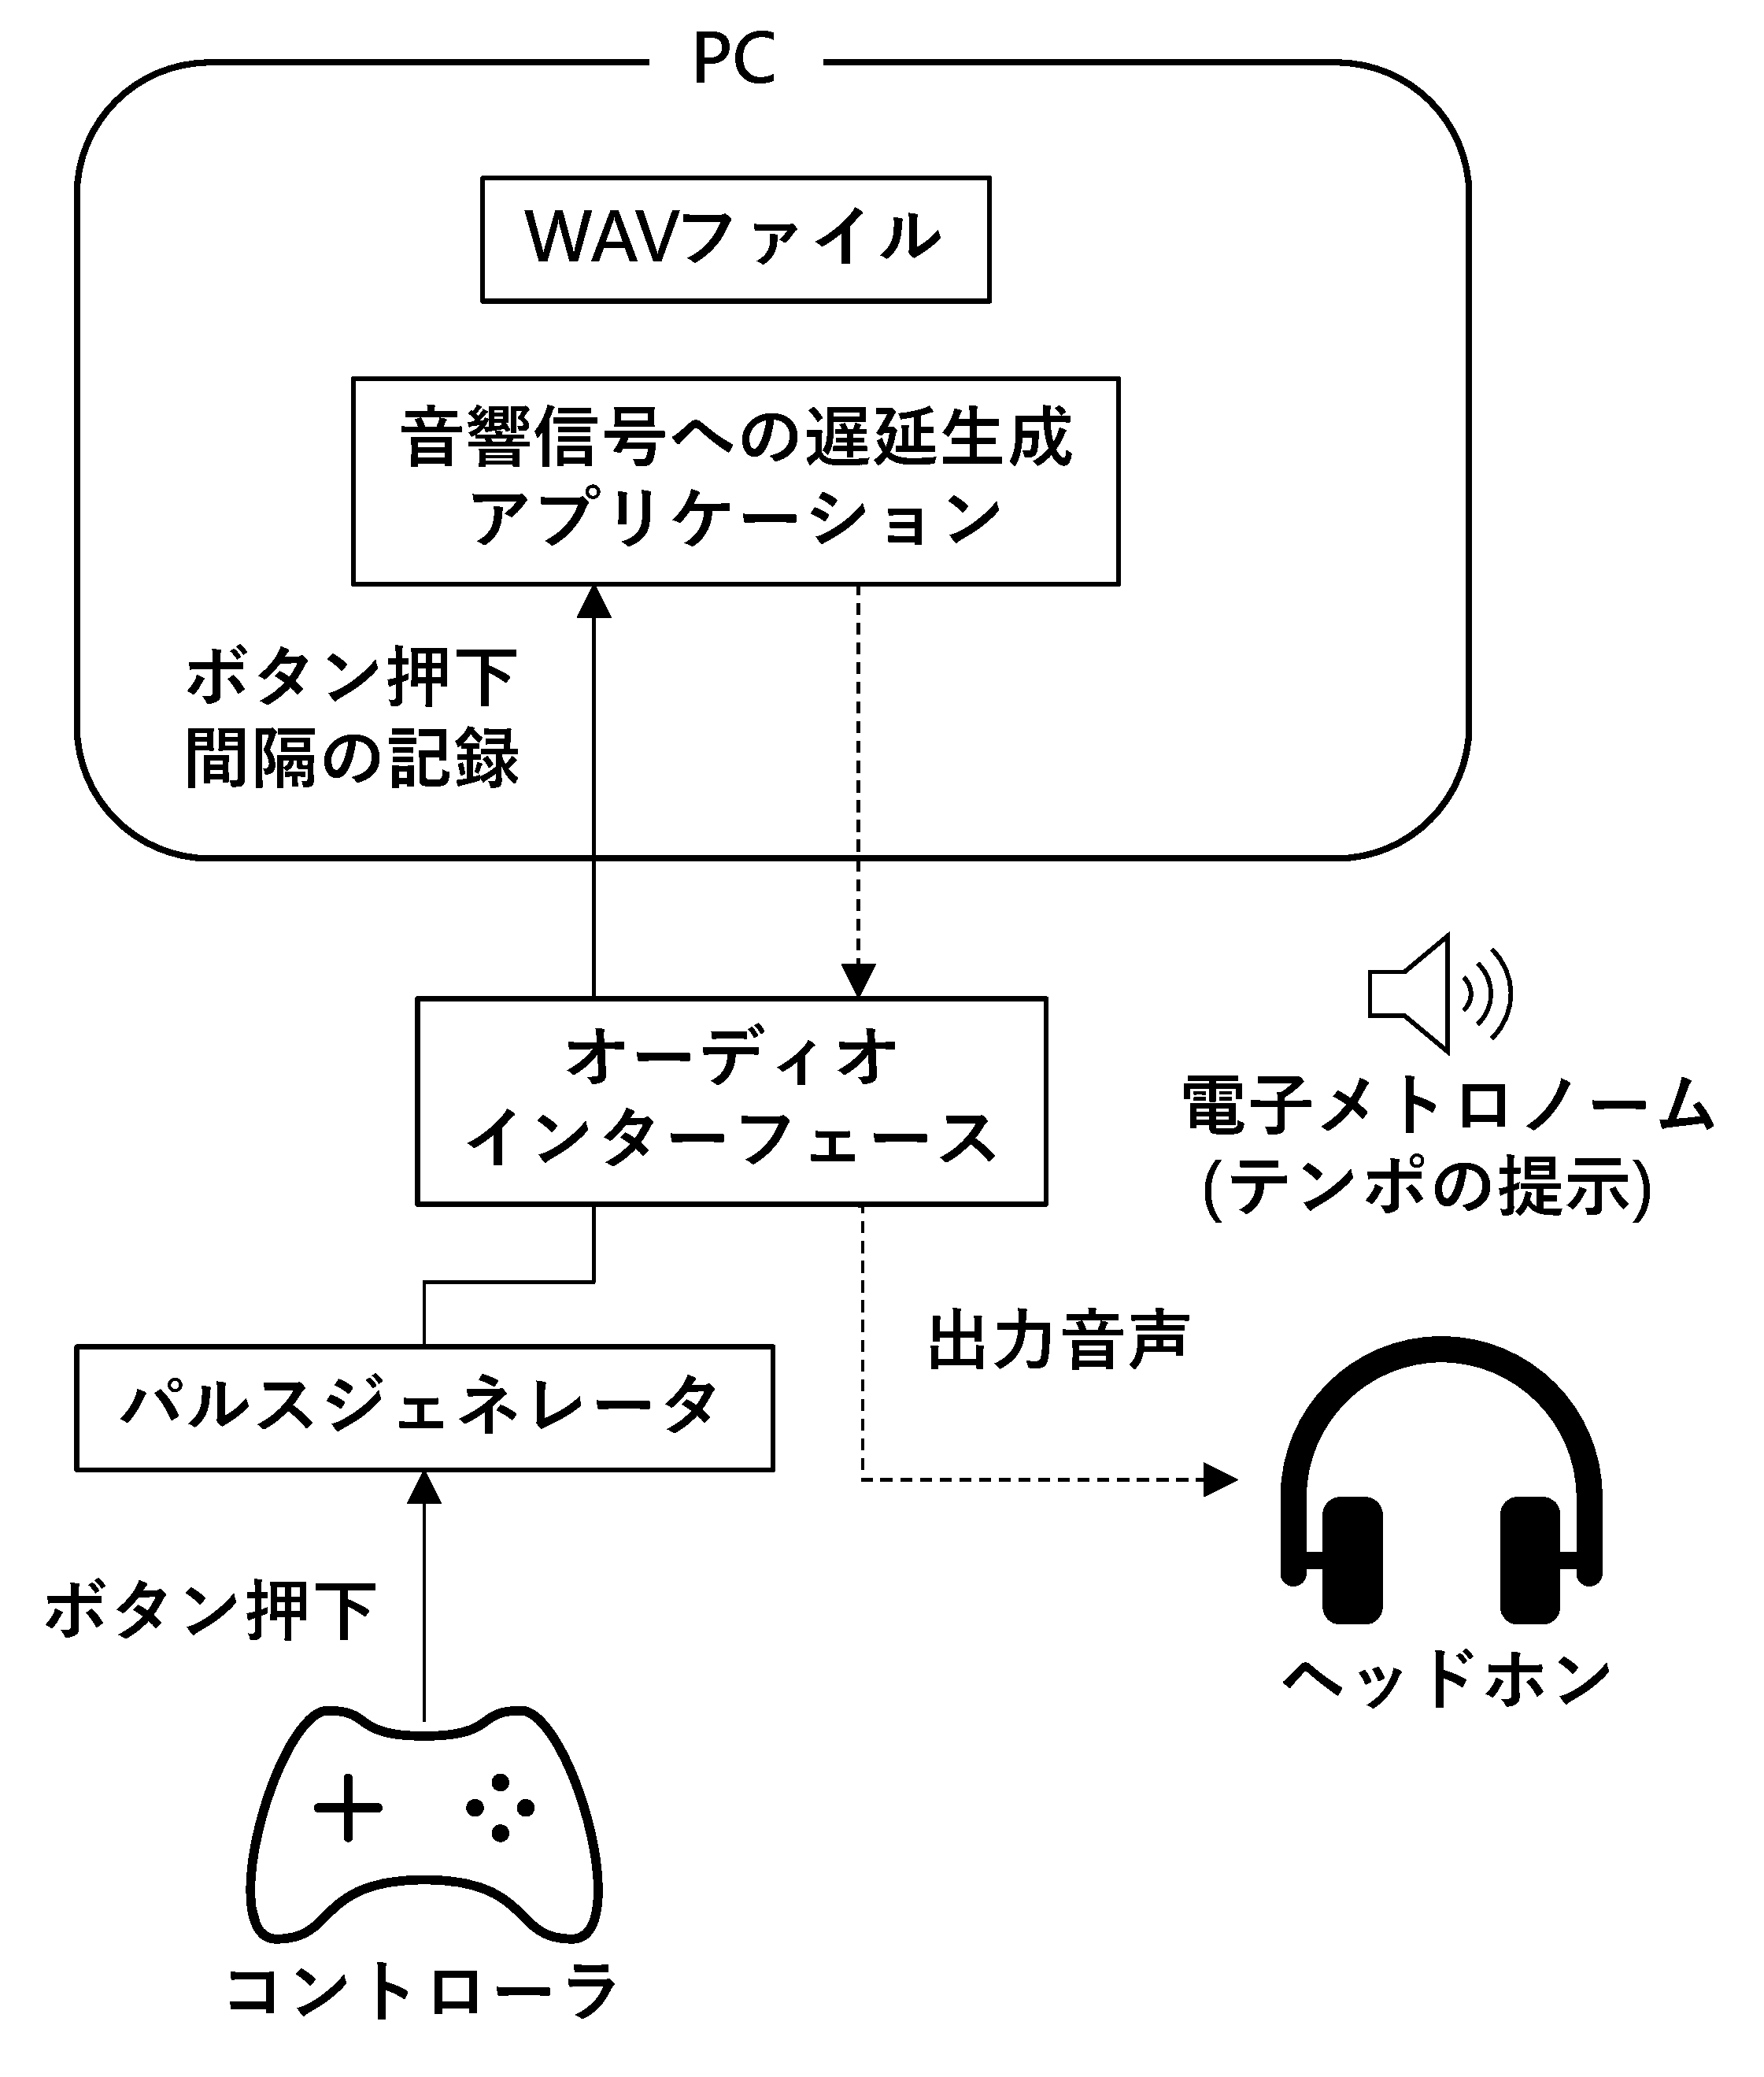
\includegraphics[scale=0.15]{figures/system_button_click.pdf}
  \caption{調査システムの構成}
  \label{fig:button-click-system}
\end{figure}
\subsection{音響信号への遅延生成アプリケーション}
本研究で使用する音響信号への遅延生成アプリケーションは,オーディオドライバにASIO(Audio Stream Input Output)を使用し,
図\ref{fig:button-click-system}に示すように,コントローラのボタンが押下されてから任意の遅延時間後にボタン押下の合図音であるクリック音のWAVファイルがヘッドホンから出力される仕組みを有している.
このアプリケーションの表示例を図\ref{fig:app_kyakkann}に示す.
\begin{figure}[tbp]
  \centering
  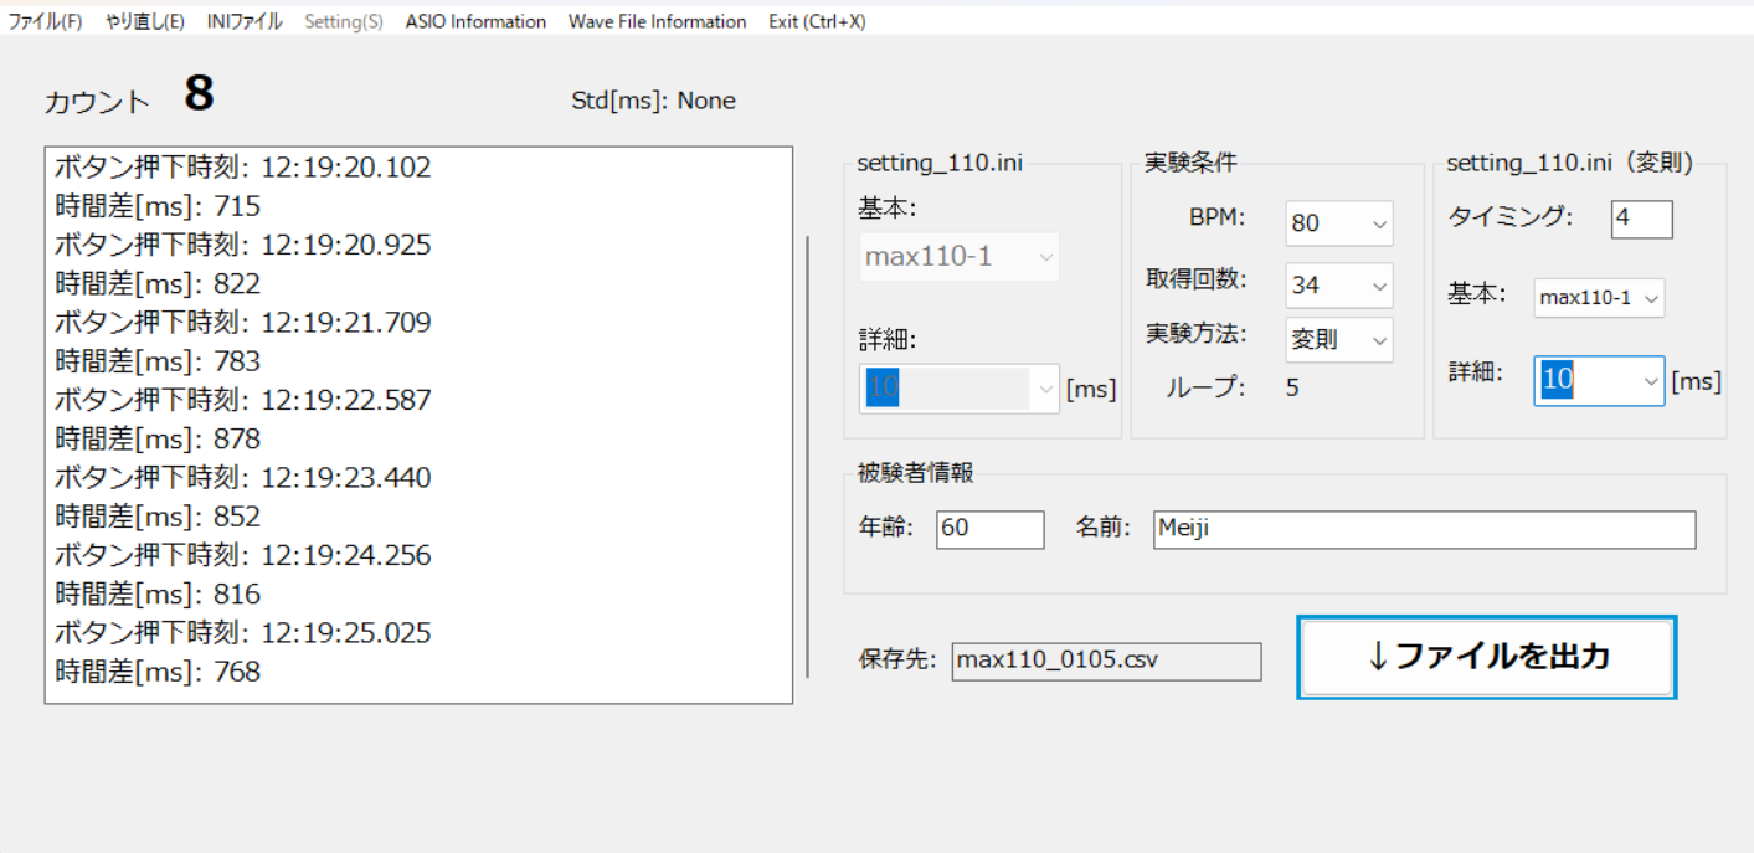
\includegraphics[scale=0.22]{figures/Apprication/App_kyakkann.pdf}
  \caption{音響信号への遅延生成アプリケーションの画面の表示例}
  \label{fig:app_kyakkann}
\end{figure}
本アプリケーションは,実験者が画面上のコンボボックスで指定した時間だけ遅延させる機能や被験者がボタンを押下する時間間隔を記録する機能を持つ.
本研究では,このアプリケーションを使用して,遅延聴覚フィードバックの身体運動への影響を調査した.